\documentclass{standalone}
\usepackage{tikz}
\usepackage{float}
\usepackage{amsmath}
\usepackage{lmodern}
\usepackage{amssymb}
\usetikzlibrary{calc}
\usetikzlibrary{hobby}
\usepackage{nicefrac}
\usetikzlibrary{decorations.markings, decorations.pathreplacing}
\usetikzlibrary{patterns, patterns.meta}
\usetikzlibrary{shapes}
\usepackage{pgfplots}
\pgfplotsset{compat=1.18}

\begin{document}

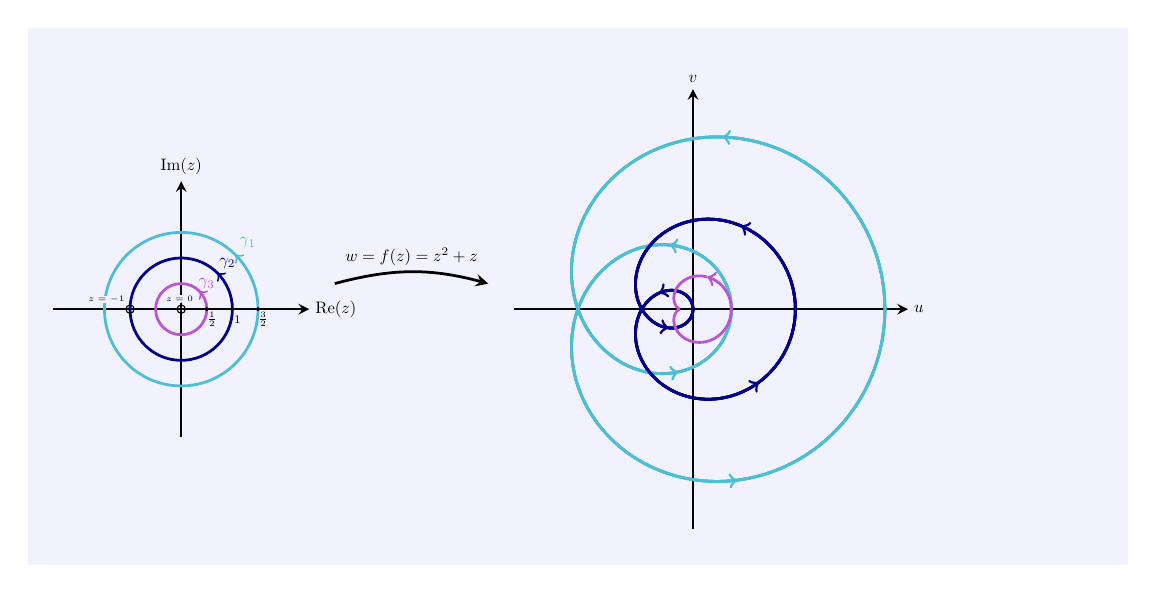
\begin{tikzpicture}[scale=0.65,
  every path/.style={line width=0.7pt}, % Thicker lines
  every node/.style={scale=0.6},         % Larger text
  arrowstyle/.style={->, >=stealth}
]

% Define the arrow decoration
\tikzset{
  arrow at angle/.style={
    postaction={
      decorate,
      decoration={
        markings,
        mark=at position #1 with {\arrow{>}}
      }
    }
  }
}

% Colors
\definecolor{gamma1}{RGB}{80, 190, 210}
\definecolor{gamma2}{RGB}{0,0,139}
\definecolor{gamma3}{RGB}{186,85,211}

\colorlet{BlueBackground}{blue!5}
% Background for entire canvas
\fill[BlueBackground] (-3,-5) rectangle (18.5,5.5);
    
% Left complex plane (z-plane)
\begin{scope}
  \draw[arrowstyle] (-2.5,0) -- (2.5,0) node[right] {$\text{Re}(z)$};
  \draw[arrowstyle] (0,-2.5) -- (0,2.5) node[above] {$\text{Im}(z)$};

  % Circles gamma1, gamma2, gamma3
  \draw[gamma1, line width=1pt, arrow at angle=0.125] (1.5,0) arc (0:360:1.5);
  \draw[gamma2, line width=1pt, arrow at angle=0.125] (1,0) arc (0:360:1);
  \draw[gamma3, line width=1pt, arrow at angle=0.125] (0.5,0) arc (0:360:0.5);

    % zeroes
  \newcommand{\DrawZero}[3]{%
    % function for drawing zeros
    % Inputs:
    % 1: coordinate (without parentheses, e.g. -1,0)
    % 2: label style
    % 3: label
    \node[solid, circle, thin, draw=black, inner sep=0pt, minimum size=5pt] (ZeroCircle) at (#1) {};
    \node[#2,font=\tiny, inner sep=0pt] at (ZeroCircle) {#3};
  }

  \DrawZero{-1,0}{anchor=south east, fill=BlueBackground, xshift=-3pt, yshift=3.5pt}{$z=-1$}
  \DrawZero{0,0}{anchor=south, ellipse, fill=BlueBackground, xshift=-1pt, yshift=3.5pt}{$z=0$}

  % Labels
  \node at (1.3,1.3) {\textcolor{gamma1}{$\gamma_1$}};
  \node at (0.9,0.9) {\textcolor{gamma2}{$\gamma_2$}};
  \node at (0.5,0.5) {\textcolor{gamma3}{$\gamma_3$}};
  \node at (0.6,-0.2) {\scriptsize $\frac{1}{2}$};
  \node at (1.1,-0.2) {\scriptsize $1$};
  \node at (1.6,-0.2) {\scriptsize $\frac{3}{2}$};
  \filldraw[black] (0.5,0) circle (0.5pt);
  \filldraw[black] (1,0) circle (0.5pt);
  \filldraw[black] (1.5,0) circle (0.5pt);
\end{scope}

% Arrow and function label
\draw[arrowstyle, line width=1pt, bend left=15] (3,0.5) to node[midway, above] {$w = f(z) = z^2 + z$} (6,0.5);
    
% Right complex plane (w-plane)
\begin{scope}[shift={(10,0)}]
  \draw[arrowstyle] (-3.5,0) -- (4.2,0) node[right] {$u$};
  \draw[arrowstyle] (0,-4.3) -- (0,4.3) node[above] {$v$};

    \newcommand{\DrawImageCurve}[3]{%
    %function for drawing poles
    % Inputs:
    % 1: circle radius
    % 2: arrow position
    % 3: curve color
    \pgfmathsetmacro{\CircleRadius}{#1}
    \pgfmathsetmacro{\ArrowPosition}{#2}
    \begin{scope} % isolates transformations
      \draw[domain=\ArrowPosition:360+\ArrowPosition,smooth,variable=\t,samples=100, #3, line width=1pt, ->]
      plot ({(\CircleRadius*cos(\t))^2 - (\CircleRadius*sin(\t))^2 + \CircleRadius*cos(\t)},
            {2*(\CircleRadius*cos(\t))*(\CircleRadius*sin(\t))+ \CircleRadius*sin(\t)});
    \end{scope}
  }

  % Parametric images of gamma1, gamma2, gamma3 under f(z) = z^2 + z
  % gamma 1
  \DrawImageCurve{1.5}{50}{gamma1}
  \DrawImageCurve{1.5}{148}{gamma1}
  \DrawImageCurve{1.5}{360-148+3}{gamma1}
  \DrawImageCurve{1.5}{360-50+3}{gamma1}

  % gamma 2
  \DrawImageCurve{1.0}{40}{gamma2}
  \DrawImageCurve{1.0}{145}{gamma2}
  \DrawImageCurve{1.0}{360-145+8}{gamma2}
  \DrawImageCurve{1.0}{360-40+8}{gamma2}


  % gamma 3
  \DrawImageCurve{0.5}{50}{gamma3}

  

\end{scope}

\end{tikzpicture}

\end{document}
